\documentclass[a4paper,11pt,twoside,dvips]{report}

\newif	\ifDraft	\Draftfalse

\usepackage{fullpage,times,graphicx,program-gh,moreverb,cite,array,ifthen}
\usepackage{disy,rcs}
\ifDraft
    \usepackage{draftcopy}
\fi
%\usepackage{changebar}
\usepackage[pagebackref,hyperindex,bookmarks]{hyperref}

%%% Fonts stuff
\renewcommand{\ttdefault}{cmtt}	% CM rather than courier
%%%

\RCS$Revision: 1.21.2.1 $
\RCS$Date: 2002/08/28 02:30:56 $

%%% graphicx stuff
\newcommand{\PicW}{0.9\textwidth}
\setkeys{Gin}{keepaspectratio=true,clip,draft=false,ext={.eps},width=\PicW}
%%% end graphicx stuff

%%% hyperref stuff
%% general setup
\hypersetup{linktocpage,colorlinks}
%% autoref labels
\renewcommand{\itemautorefname}{Item}
\renewcommand{\chapterautorefname}{Chapter}
\renewcommand{\sectionautorefname}{Section}
\renewcommand{\appendixautorefname}{Appendix}
\renewcommand{\subsectionautorefname}{Section}
\renewcommand{\subsubsectionautorefname}{Section}
\renewcommand{\Hfootnoteautorefname}{Footnote}
%% Commands for index
\newcommand{\Htextbf}[1]{\textbf{\hyperpage{#1}}}
%%% end hyperref stuff\index{stuff}


\begin{document}
\ifDraft
   \newcommand{\DraftComment}[1]{{\bf\em #1}}
   \newcommand{\draftComment}[1]{\textbf{\emph{#1}}}
\else
   \newcommand{\DraftComment}[1]{\relax}
   \newcommand{\draftComment}[1]{\relax}
\fi
\newcommand{\Note}[1]{\par{\bf Note:} #1\par}
\newcommand{\Raise}[1]{&\multicolumn{2}{@{} l |}{|\RAISES #1|}}
\newcommand{\Fails}[1]{&\multicolumn{2}{@{} l |}{|\FAILS #1|}}
\newlength{\FailsLng}
\newcommand{\FailS}[1]{&\multicolumn{2}{@{} l |}
              {\settowidth{\FailsLng}{|\FAILS |}\hspace{\FailsLng}|#1|}}
\newcommand{\Never}{&\multicolumn{2}{@{} l |}{\bf never fails}}
\newcommand{\Ret}{\(\AR\)}			% ``returns'' for functions
\newcommand{\Cite}[1]{\relax}	% for references to be added in final version
\renewcommand{\topfraction}{0.95}
\renewcommand{\bottomfraction}{0.95}
\renewcommand{\textfraction}{0.05}

\pagenumbering{roman}
%\sloppy

\title{The Mungi Kernel API}
\author{Version 1.2}
\date{\ifDraft Draft of \fi\RCSDate\ifDraft, document revision \RCSRevision\fi}
\maketitle
\thispagestyle{empty}
\pagestyle{headings}

\vfill
\begin{abstract}
\setcounter{page}{2}
This document describes version 1.2 of the application
programming interface to the kernel of the \emph{Mungi}
single-address-space operating system. This interface will, in general,
only be used by low-level software, most applications are expected to
use a higher-level interface implemented as system libraries. Such
libraries will be described in separate documents.

\vfill
\noindent\hrulefill\\
%
Copyright \copyright~2002 by Gernot Heiser, The University of New
South Wales.\\
Permission is granted to copy, distribute and/or modify this document
under the terms of the GNU Free Documentation License, Version 1.1,
published by the Free Software Foundation; there
being no Invariant Section, no Front-Cover Texts and no Back-Cover
Texts.  A copy of
the license is included in \autoref{a:license} entitled ``GNU Free
Documentation License''.\\[2ex]
%

\end{abstract}

\setcounter{page}{3}
\tableofcontents

\cleardoublepage
\setcounter{page}{1}
\pagenumbering{arabic}
%\thispagestyle{empty}

\chapter{Introduction}

Mungi~\cite{Russell_SEHBGH_92, Heiser_ERH_93:tr,
Vochteloo_RH_93, Heiser_ERV_94, Elphinstone_RHL_96, Vochteloo_ERH_96,
Heiser_EVRL_98, Deller_Heiser_99} is a single-address-space
operating system (SASOS)~\cite{Chase_LFL_94, Wilkinson_MRHL_95:tr}
developed by the Operating Systems and Distributed Systems Group at the
University of New South Wales. It is conceptually similar to
Angel~\cite{Wilkinson_SGWOSK_92, Wilkinson_Murray_96} and
Opal~\cite{Chase_LBL_92, Chase_LFL_94}, although quite different in many
important aspects. Most notably, Mungi presents the single-address-space
model in a very pure form, as it provides no
inter-process-commu\-ni\-cation mechanisms other than shared
memory. Many of the basic ideas in Mungi go back to the IBM
System/38~\cite{Berstis_80, Houdek_SH_81} and its successor, the
AS/400~\cite{Soltis:as400}.

This document presents the application programming interface (API) of
the Mungi kernel. While Mungi does not pretend to be a microkernel (in
fact, the prototype is implemented on top of the L4
microkernel~\cite{Liedtke_95}), it nevertheless presents a minimal and
low-level interface to the programmer. Policies are, as far as possible,
left to be implemented by higher software layers. Similar to
microkernels, Mungi allows the implementation of device drivers and page
fault handlers at user level.

As a consequence, application programs will not normally interface
directly to the Mungi kernel, but are expected to call a higher level
library interface. A UNIX-like interface has partially been developed,
however this will be described in a separate document.

The following sections list and explain the Mungi system calls. These
are presented in (hopefully) intuitive pseudocode. The actual C language
bindings are presented in the Appendix.

\section{\label{s:conv}Conventions}

This document presents Mungi system calls and data structures in an
abstract format, showing the main characteristics but not detailed type
information etc. Consult the C language bindings in
\hyperref[s:h]{Appendix~\ref*{s:h}} for actual types and syscall
signatures.

The system call tables show possible failure modes of various calls. An
error condition is indicated by the syscall returning a value indicating
failure, the syscall |GetLastError()| can then be used to obtain the
actual error number.

\iffalse
\section{TO DO:}

\begin{itemize}

\item \draftComment{Check bank account permissions}

\item \draftComment{Check PDX params}

\end{itemize}
\fi



\chapter{\label{s:obj+caps}Objects and Capabilities}

Objects are Mungi's storage abstraction, they are the unit of virtual
memory allocation and protection. Objects are page aligned and consist
of an integral number of pages. Newly allocated objects are zero
filled. From the system's point of view, an object is simply a
contiguous, aligned region of virtual address space; the system imposes
no structure on objects (but higher software levels are free to do
so). Access to objects is controlled by \emph{password
capabilities}~\cite{Anderson_PW_86}.

\section{\label{s:caps}Password capabilities}

\begin{figure}[htb]
\begin{center}
\includegraphics[width=0.48\textwidth]{cap}
\end{center}
\caption{\label{f:cap}Format of a capability}
\end{figure}

\autoref{f:cap} shows the format of a capability. The virtual page
number refers to the base address of an object. The mode indicates the
rights conferred by the capability. This field is only a hint for the
user, it is ignored by the system when a capability is presented. The
system maintains a directory, the \emph{object table} (OT), of object
attributes, including the set of valid passwords and their corresponding
modes.

There are five different rights capabilities may grant over an object:
read (R), write (W), execute (X), destroy (D), and \emph{protection
domain extension} (PDX); the latter will be explained in
\autoref{s:pdx}. Each valid capability grants the holder a combination
of these rights to an object.\footnote{Note that, as we are relying on
the hardware to enforce protection, on many architectures we cannot
guarantee that a user cannot read an object to which they only hold an X
capability.} A capability granting RWXD rights is, by definition, an
owner capability. A capability containing a zero password is considered
a valid capability granting no access rights.

Capabilities can confer negative rights (\emph{negative
capabilities}). These can be used to ensure that a client does
\textbf{not} have certain access rights. For example if, while
validating an attempted write access, the system encounters a \emph{not
write} capability, it will raise a protection fault. A negative
capability is indicated by a |NOT| bit in the mode field. If this bit is
set, the capability negates the rights indicated by the other rights
bits.

Capabilities are user objects and can be stored and passed around
freely. They are protected from forgery by sparsity, hence careful
choice of passwords is important. The system provides a library routine
to create random passwords.

As capabilities are user objects, it is not possible to determine who
has access to a particular object. It is also normally impossible to
prevent a particular user, who has been given a capability for an
object, from handing this capability to other users. However, the
|ObjPasswd| call allows revocation of a capability.
Furthermore there exist a mechanism for confining clients of one's
objects, see \autoref{s:confine}.



\section{\label{s:sp-obj}Special objects}

Some objects are of a \emph{special} nature in the sense that certain
system calls require a reference to such objects, and the system must be
able to guarantee that such objects can only be created by authorised
agents.

Presently there are two types of special objects: \emph{bank accounts}
and \emph{protection domains}. The former constitute the basic mechanism
for resource accounting in Mungi, while the latter support creation of
threads with access rights different from the caller's.

The use of bank accounts for resource management is discussed
in~\cite{Heiser_LR_98}. The support provided by Mungi is to make bank
accounts special and to ensure that every object created has an
associated bank account. The use of protection domains is further
explained in \autoref{s:pd}.

What makes an object special is an association with a \emph{controlling
object}. The system protects speciality by only allowing a thread to
make an object special \emph{if the thread has read access to the
controlling object}. The type of the controlling object must agree with
the speciality type requested for the controlled object. Special objects
whose controlling object no longer exists are cleaned up by the system
lazily.

An object which is its own controlling object is a \emph{master object}
for a type of special objects. Creation of master objects requires
special privilege (read access to the \emph{object table}).

Special objects are not executable code, and the execute permission bit
takes on a special meaning for these objects: It allows the holder to
use the object (charge an object's storage to a bank account, start a
thread in a protection domain) without being able to read the object's
data.


\section{\label{s:ot}Object descriptors}

\autoref{t:info} shows the format of an object descriptor which is
used to describe object attributes. That descriptor format is used when
inquiring or setting object attributes in the OT.
\begin{figure}[htb]
\begin{center}
\begin{programbox}
\TYPE |ObjInfo| \BODY \{
	\COMMENT{public part}
	|length|, |extent|,
	|create\_time|, |modify\_time|, |access\_time|, |accounting\_time|,
	|user\_info|, |accounting\_info|,
	\COMMENT{restricted part}
	\{ |password|, |mode| \} [|n_caps|],
	\{ |clist\_cap|, |password|, |entry\_pt| [|n_entry|] \} [|n\_pdx|],
	|bank\_acct\_cap|, |pager\_cap|, |flags|,
	|special|, |controlling\_cap|
\ENDTYPE\}
\end{programbox}
\caption{\label{t:info}Object descriptor (|info|) data structure.}
\end{center}
\end{figure}
The meaning of the
fields is as follows:
\begin{description}
\item[|length|:] length of the object in bytes. The system will round
this to a multiple of the basic hardware page size (or bigger) and will
also take into account the |extent| value.
\item[|extent|:] unit of backing store allocation. The system rounds
this to an integer multiple of the page size (which may be the next bigger
integer multiple, or the next bigger power-of-two multiple). The system may
ignore changes to the original setting.
\item[|create\_time|, |modify\_time|, |access\_time|:] timestamp of
object creation, last modification, last access. The modification and
access time stamps are automatically updated by the system (with limited
accuracy).
\item[|accounting\_time|:] timestamp used by the accounting system.
\item[|accounting\_info|:] reserved for usage by accounting system.
\item[|user\_info|] a user-defined field which may be used, e.g., for
implementing a type system on top of the Mungi kernel. The system does
not use this field, but ensures that only an owner can change it.
\item[|password, mode|:] list of non-PDX passwords plus access rights
conferred by each password.
\item[|clist\_cap|:] Clist capability for extending the APD when the
object is invoked via the |PdxCall| system call (c.f.\ \autoref{s:pdx}).
\item[|password, entry\_pt{[]}|:] list of passwords allowing PDX call,
plus the set of entrypoints allowed for each password.
\item[|bank\_acct\_cap|:] R capability to the \emph{bank account} to
which storage costs for the object is charged. Bank accounts are the
basis of Mungi's management of memory resources. The kernel only
provides the mechanism by ensuring that a bank account is associated
with every object, and by protecting bank accounts from forgery. The
operation of the accounting system is described
in~\cite{Heiser_LR_98}.
\item[|pager\_cap|:] PDX capability to the page fault handler for the
object. Null if handled by the default pager.
\item[|flags|:] array of other object attributes. Present values:

\begin{description}
%\item[|sharable|:] indicates that the object can be shared with
%other tasks. If set, the object may be accessed by any thread whose
%protection domain contains a valid capability to the object. If not set,
%the object may be unaccessible by others even if they hold a valid
%capability. Unshared objects may be cheaper to create and destroy. The
%system may use the initial setting of this flag as a hint to direct the
%allocation strategy. The flag can be turned on at any time. The system
%may ignore attempts to turn it off.
\item[|persistent|:] indicates that the object may outlive its
creator. An object created with this flag off will be cleaned up by the
system when the creator thread exits. The flag can be
turned on by an owner, however, this may have no effect if called from a
thread running in an APD different from the creator's.
The flag can be turned off by an owner, in which case the object is
marked for cleanup when the caller's thread exits. Object
cleanup may be delayed if the exiting thread is the descendent of
another thread running in the same APD.
\end{description}
\item[|special|:] array of flags identifying special object
types. An attempt to change any of these will only be honoured if the
controlling object is not-null (or being made not-null at the same
time), the caller has read access to the controlling object and the
controlling object has the corresponding bit set. Present values:
\begin{description}
\item[|is\_acct|:] indicates that the object can be used as a \emph{bank
account}.
\item[|is\_financial|:] indicates that the bank account object can
presently be used for object creation.
\item[|is\_pd|:] indicates that the object can be used as a
\emph{protection domain}.

\end{description}
\item[|controlling\_cap|:] specifies that the object is \emph{special}
and has the specified \emph{controlling object}. An attempt to change
the controlling object attribute will only be honoured if the caller has
read access to that controlling object and the latter is
\emph{special}. An object can be made its own controlling object if the
caller has read access to the object table.
\end{description}



\section{System calls}

System calls dealing with objects are summarised in
\autoref{t:obj_cap} and explained below.

\begin{table*}[htb]
\begin{center}
\begin{tabular}{| l @{ } l @{ } l |}\hline
\multicolumn{3}{|l|}{System calls:}\\\hline
|ObjCreate|	&(|size, password, info|)	&\Ret(obj\_adr)\\
	\Fails{invalid\_info, out\_of\_memory, invalid\_bank\_account}\\
|ObjDelete|	&(|adr|)			&\\
	\Fails{protection\_violation}\\
|ObjResize|	&(|adr, new\_size|)		&\\
	\Fails{protection\_violation, invalid\_info, cannot\_grow, out\_of\_memory}\\
|ObjNewPager|	&(|adr, pager|)	&\\
	\Fails{protection\_violation, invalid\_PDX}\\
%\hline\hline\multicolumn{3}{|l|}{Library calls:}\\\hline
|ObjPasswd|	&(|cap, mode|)	&\\
	\Fails{protection\_violation, table\_overflow}\\
|ObjCrePdx|	&(|cap, clist, n\_entries, entry[]|)		&\\
	\Fails{protection\_violation, table\_overflow, invalid\_PDX,}\\
	\FailS{invalid\_Clist, invalid\_NULL\_value}\\
|ObjInfo|	&(|adr, update\_flags|, OT\_entry)	&\Ret(|OT\_entry|)\\
	\Fails{protection\_violation, invalid\_info}\\
\hline
\end{tabular}
\end{center}
\caption{\label{t:obj_cap}System calls dealing with objects and capabilities.}
\end{table*}



\begin{description}
\item[|ObjCreate|:] allocates a new object of a specified |size|. The
call returns the base address of the object. Together with the
password supplied by the caller, this will make an \emph{owner
capability} for the new object. The caller supplies an optional
|ObjInfo| data structure (to which they must have read access) which is
used to initialise the object
descriptor in the OT. The fields used are |bank\_acct\_cap|, |extent|,
|user\_info|, |flags|, |special| and |controlling\_cap|, other entries
are ignored. Setting |special| and |controlling\_cap| requires special
privilege as explained above. If the |bank\_acct\_cap| is not given (or
no |info| parameter supplied) the caller's default bank account is
used.

The system may use some of the data in |info| as a hint to optimise its
allocation strategy.

Initially, all page faults on the object are handled by the
\emph{default pager}, which initialises pages to zero. Note that a newly
created object is not accessible until entered into a Clist.

\item[|ObjDelete|:] deallocates the object containing |adr|. The
caller's protection domain must contain a destroy capability for the
object, or must have execute access on the object's bank account. Virtual
memory previously allocated to that object may be reused for objects
created in the future, hence it is important that passwords cannot be
guessed.  Reuse of virtual memory will only happen once it is certain
that no validations are still cached.

\item[|ObjResize|:] expands or shrinks the object containing |adr| to
|new\_size|. An object may not be able to grow if the following address
space has already been allocated to a different object; a |cannot grow|
exception will be raised in this case. The caller's protection domain
must contain an owner capability for the object.

\item[|ObjNewPager|:] registers a new page fault handler for the object
containing |adr|. A null |pager| address reverts to the system's default
pager. The caller's protection domain must contain an owner capability
for the object. Executing this system call implies calling
|PageUnmap(base,length,zero)| on the object. See \autoref{s:page} for
details.

\item[|ObjPasswd|:] registers a new capability for an object, or removes
an existing one for the object referred to by |cap|. A capability is
deleted by specifying its password and a null |mode|. The |mode|
parameter specifies the strength of that capability. If |mode| is RWXD,
the new capability is an owner capability, conferring the same rights as
the original owner capability. The PDX bit, if set in |mode|, is
ignored. The caller's protection domain must contain an owner capability
for the object.

\item[|ObjCrePdx|:] registers a new PDX capability for the object
referred to by |cap|, together with the protection domain extension (one
Clist) and a list of valid entry points for which that password can be
used. The caller's protection domain must contain an owner capability
for the object, and at least execute rights to the Clist.

If a PDX password for this object has been registered before,
|clist\_cap| will overwrite any protection domain extension previously
registered, except if null, in which case the protection domain
extension remains unchanged. If the same PDX password has been
registered for the object before, the list of entry points for that
password will be reset to the one specified. However, if |n\_entries| is
negative, the list of entry points will not be changed. If |n\_entries|
is zero, the password will be revoked as a PDX password.

The call fails if no protection domain extension is registered at all,
i.e.\ if an attempt is made to register the first PDX password with
|clist\_cap| being null or |n\_entries| being less than or equal to zero.

PDX procedures are described further in \autoref{s:pdx}.

\item[|ObjInfo|:] updates the object descriptor in the OT for the object
containing |adr|, requires at least read or execute rights on the
object. The system ignores all passwords as well as the |pager|
field. |update\_flags| specify which attributes are to be updated.  An
attempt to set |extent| may be ignored. Returns the previous value of
the object descriptor. Passwords are returned if called by an owner,
otherwise passwords will be returned as zeros.

% Should we have a meta-right only for ObjInfo??? YES

The |controlling\_cap| is only set if \emph{all} of the following
conditions are met:
\begin{itemize}
\item the controlling capability was null before the call, or the caller
has read access to the old controlling object,
\item the new controlling capability is null or the caller has read
access to the new controlling object,
\item the new controlling object is of the same |special| type as the
target object is to become.\footnote{Note that it is not sufficient for
|controlling\_cap| to be valid for read access, the read access must be
allowed by the caller's active protection domain see \autoref{s:apd}.}
\end{itemize}

If the caller has owner rights, |bank\_acct\_cap|, if given, is
validated and used as the new bank account, otherwise this field is also
ignored.

Time stamps may be updated by setting an appropriate bit in
|update\_flags|. The table below gives the minimum amount of privilege
required for the various operations possible. Here \emph{touch} means
setting a time stamp to the present time and date, while \emph{set}
means setting to an arbitrary time and date. The \emph{R-OT} privilege
means that a R capability for the OT is required (note that this implies
RWXD capability on any object). As usual, \emph{RWXD} stand for an owner
capability, \emph{W} is a capability which allows write access, while
\emph{R/X} means a capability allowing read \emph{or} execute
access. The creation timestamp cannot be changed.
\begin{center}
\begin{tabular}{l  r r}
\em Time stamp		& \multicolumn{2}{c}{\em min.\ privilege for}\\
			& \em touch		& \em set \\ \hline
modification		& W			& RWXD \\
access			& R/X			& RWXD \\
accounting		& R-OT			& R-OT \\
\end{tabular}
\end{center}
\end{description}





\chapter{\label{s:pd}Protection Domains}

In general, a thread's protection domain is its set of
access rights to objects. In a capability system, this is equivalent to
a set of capabilities.

Mungi's protection system has been designed to be unintrusive, hiding
its operation from applications as far as possible. For this reason,
Mungi does not expect capabilities to be presented explicitly when an
object is accessed. Instead, users store their capabilities in a
datastructure which is searched by the kernel when an access validation
needs to be performed. This datastructure is called a thread's
\emph{active protection domain} (APD).

A new thread is created by the parent performing a
|ThreadCreate| system call. That call takes a parameter |pd| which
indicates the protection domain in which the new thread is to
execute. If the |pd| parameter is null, the new thread \emph{shares},
for its lifetime, the parent's protection domain.  Otherwise the thread
is created in its own APD. The APD is in this case instantiated from a
template \emph{protection domain object} referenced by the |pd|
parameter. A flag determines whether the new thread may join the APD of
another thread whose APD has been instantiated from the same PD
object. The system ensures that, if it allocates a stack object for a
thread running in a newly created APD, capabilities to the stack object
are inserted into the APD (see \autoref{s:proc-mod} for
details).

\section{\label{s:pdo}Protection domain objects}



A \emph{protection domain object} (PD object) is a special object with
the |is\_pd| flag set. It is used to describe a protection domain in
which threads can be created. The structure of a PD object is:


\begin{center}
\begin{programbox}
\TYPE |apddesc| \BODY \{
	|clist|[|n\_pd|], |n\_locked|;
\ENDTYPE\}
\end{programbox}
\end{center}

Here, |clist| is a capability for a \emph{capability list} (Clist) and
|n\_locked| specifies the number of locked slots in the APD. The
semantics of these fields is described in Sections~\ref{s:apd} and
\ref{s:apdlock} below. Note that the first entry in the |clist| array
will be overwritten on use and should therefore be left empty.

When a thread is created with a valid non-null |pd| parameter, a new APD
is created for the thread. The new APD is a copy of the PD object
referenced by the |pd| parameter. For more details see
\autoref{s:thread}.


\section{\label{s:apd}Active protection domains}

A thread's APD is represented by the same information as what is found
in a PD object. The |apddesc| data structure is kept in kernel space as
part of the internal thread description. The actual Clists are user
objects (and, as such, themselves parts of protection domains), as shown
in \autoref{f:apd}.

\begin{figure*}[htb]
\begin{center}
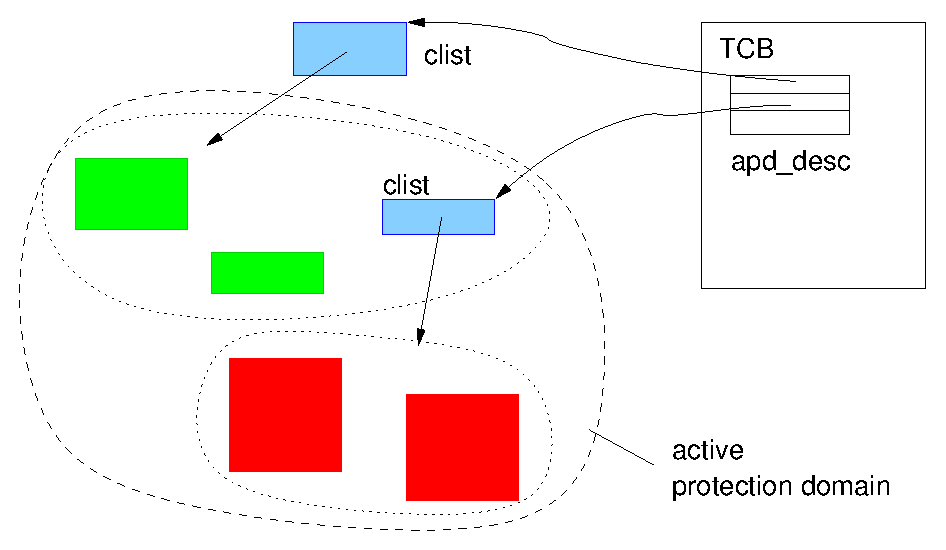
\includegraphics[width=0.7\textwidth]{APD}
\caption{\label{f:apd}Active protection domain.}
\end{center}
\end{figure*}

Clists are user-maintained datastructures in a standard format. Users
can, protection permitting, add or remove capabilities in their Clists
at any time without system intervention. Addition or
removal of Clist capabilities to a running thread's APD is possible via
the |ApdInsert| and |ApdDelete| system calls. Such an operation will
affect all threads sharing an APD.

\begin{figure*}[hbt]
\begin{center}
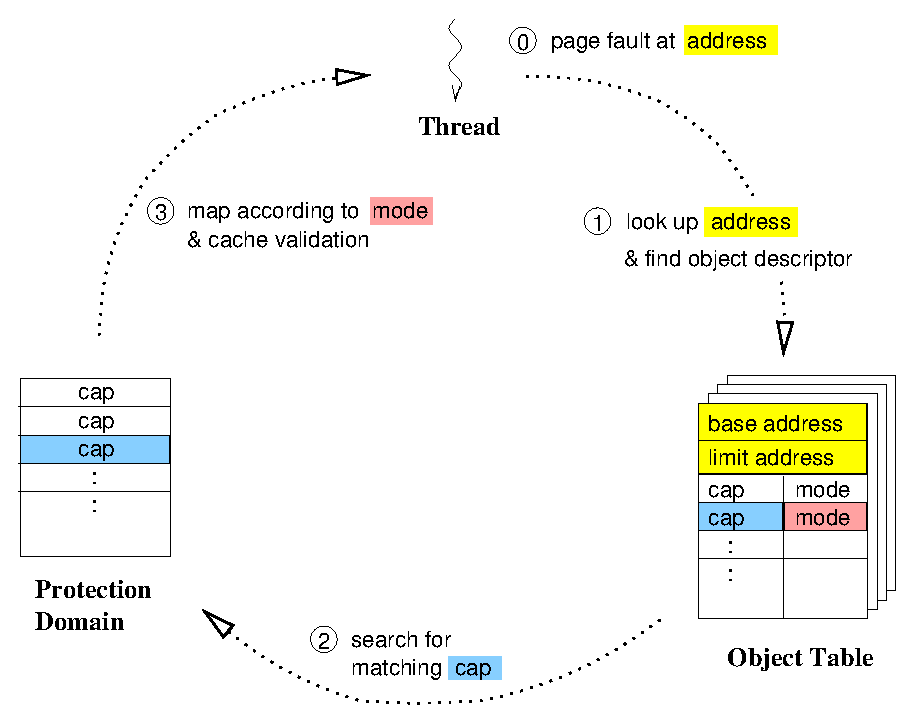
\includegraphics[height=0.4\textheight]{validate}
\caption{\label{f:valid}Access validation.}
\end{center}
\end{figure*}


Validation of an access is normally performed by the system in response
to a protection fault, i.e., an object was accessed for which the kernel
does not have information on the validity of the access, or that
information is inconsistent with the mode of the access. In order to
perform the validation, the system searches the OT with the faulting
address. If no matching object is found, a protection fault is
signalled to the user thread.  Otherwise, the APD is searched for a
capability matching one of those in the OT with appropriate mode. If
found, a mapping for the object is established and the validation
information is cached by the kernel to avoid having to validate each
page of a large object individually. The validation process is depicted
in \autoref{f:valid}. The basic algorithm is shown in
\autoref{f:valid-alg}.

\begin{figure}[htb]
\begin{center}
\begin{programbox}
\FUNCT |validate|(|fault\_adr|, |mode|) \BODY
   \IF \NOT |OT\_lookup| (|fault\_adr|\RETURNS|base|, |limit|, |caps|) \THEN
	\RAISE |protection violation|;
   \FI;
   \FOR |i| = 0 \TO |apd.n_pd-1| \DO
	    \FOREACH |c| \in |apd.clist[i]| \DO
		\IF |c| \in |caps| \AND |c.negative| \AND |mode| \supseteq |c.mode| \THEN
			\RAISE |protection violation|;
		\ELSIF |c| \in |caps| \AND |mode| \subseteq |c.mode| \THEN
			\RETURN (|base|, |limit|, |c.mode|);
		\FI;
	    \OD;
\OD;
\RAISE |protection violation| \ENDFUNCT
\end{programbox}
\end{center}
\caption{\label{f:valid-alg}Access validation algorithm.}
\end{figure}

As the validation algorithm shows, the search is terminated when the
first (positive or negative) capability of sufficient
strength is found. Users can use this to arrange their capabilities such
as to avoid double validation faults.

Presently there are two Clist formats, an unsorted one and one where
capabilities are sorted by object base address. The kernel uses binary
search on sorted Clists.

Any invalid (as opposed to negative) capabilities
encountered while searching the APD are ignored. This avoids race
conditions with newly created capabilities, and synchronisation problems
problems if validation occurs concurrently with Clist updates. Searching
a (due to updates) inconsistent ``sorted'' Clist may fail to locate an
existing capability.  Users are therefore responsible for setting the
format indicator to ``unsorted'' before adding or removing capabilities
in a Clist.\footnote{Note that this scheme cannot completely prevent
such failures. However, we expect that sorted Clists are modified very
infrequently. The extremely rare chance of a transient failure to locate
a capability does not seem to justify the expense of proper concurrency
control. Paranoid users can, of course, replace the whole Clist, which
can be done without ever leaving an inconsistent Clist in the APD.}
The search order \emph{within} a Clist is undefined.

Caching of validations could delay the effect of revocations of
passwords indefinitely. To prevent this, the system guarantees that no
validations are cached for more than a certain amount of time. Clist
capabilities in the APD are also periodically revalidated; if such a
capability is found to have become invalid it is silently removed from
the APD.

\section{\label{s:pdx}Protected procedure calls}

Mungi provides a protected procedure call mechanism similar to the
\emph{profile adoption} mechanism of the IBM
System/38~\cite{Berstis_80}. Mungi's mechanism, called \emph{protection
domain extension} (PDX) allows the caller of a PDX procedure to change
its protection domain, for the duration of the call, in a controlled
fashion.

More specific, a PDX procedure has, in the object table, registered a
set of valid entry points and a capability for a Clist (c.f.\
\autoref{s:ot}). When a |PdxCall| system call is executed, the system
first verifies that the caller possesses a valid PDX capability and
tries to access a valid entry point, then extends the caller's APD by
the PDX's Clist, and finally transfers control to the PDX code. When the
PDX procedure returns, the PDX Clist (and all cached validation
information relating to that Clist) is removed from the caller's
APD. Note that for the duration of the PDX call, the calling thread's
change of protection domain does not affect other threads executing in
the caller's APD --- such threads have no access to the called object
(unless they also perform an appropriate PDX call).

\begin{figure}[htb]
\begin{center}
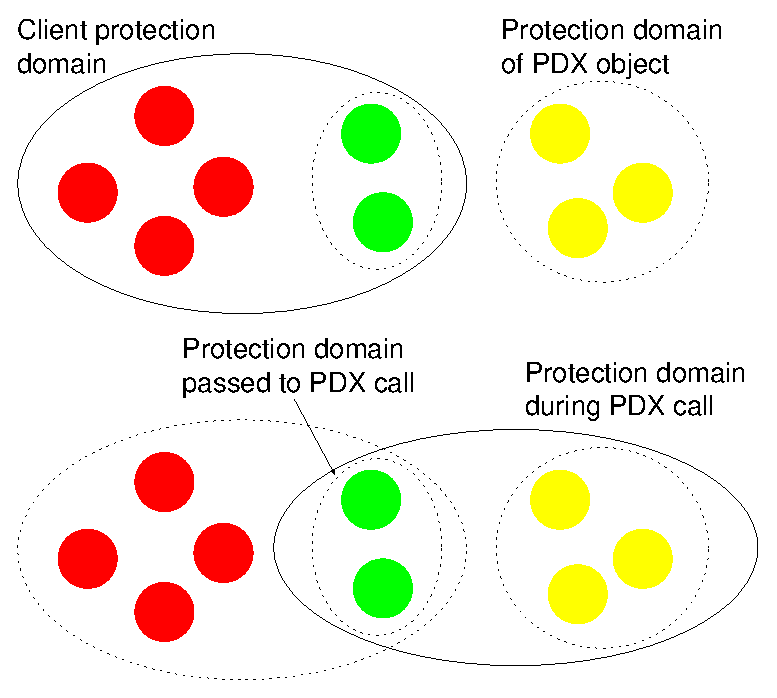
\includegraphics[width=0.5\textwidth]{PDX}
\end{center}
\caption{\label{f:pdx}Active protection domains during a PDX call.}
\end{figure}

Instead of having the PDX procedure execute in a superset of the
caller's protection domain, the caller has the option of explicitly
supplying a protection domain object reference when
calling the PDX procedure. In this case, the call executes in a
protection domain which is the union of the supplied one with that
registered for the PDX object. This is shown in \autoref{f:pdx}.

The ability of passing a protection domain gives the caller maximum
control over which objects the PDX procedure can access. In particular,
an empty protection domain may be passed to the PDX procedure, the
latter then has no access to any of the caller's data (other than
by-value parameters). Note that it is also possible to pass a capability
(say for a result buffer) on the call explicitly; the PDX procedure must
then insert that capability into one of its Clists.

\section{\label{s:confine}\label{s:apdlock}Discretionary confinement}

Since the APD data structure contains actual capabilities for
Clists, there is no need for Clist capabilities to be contained in any
of a thread's Clists. As Clist capabilities are immediately validated
when added to the APD, the system can rely on all Clists referenced by
the APD to be accessible. A thread holding no read capability to any of
its Clists can use the Clists to access objects, but cannot look at the
capabilities contained in the Clists themselves.

Applications can make use of this to \emph{confine} untrusted
code. Mungi provides the facility of \emph{locking} part or all of a
thread's APD. Locked Clist capabilities cannot be changed or removed,
and no new Clist capabilities can be added before them. This also
applies to the (implicit) addition of Clist capabilities during a PDX
call --- PDX Clist capabilities will only be inserted into the caller's
APD \emph{after} any locked slots. A thread whose APD is defined by
Clists which are all outside the APD, and whose APD is locked, has no
way to modify its APD.

A thread with a locked APD, and with no write capabilities to objects
readable by others, is unable to leak any of the data it has access
to. A partially locked APD does not confine a thread, but can ensure
that certain objects remain unaccessible, provided that one of the
locked Clists contains sufficient \emph{negative} capabilities to the
objects which are not to be accessed\cite{Vochteloo:phd}. Note that this
form of confinement can only work because all capability presentation
is implicit.

\begin{sloppypar}
The system libraries contain a procedure which, using one-way functions,
generates reduced-strength capabilities from a given capability. While
usage of this method is not enforced by the system, using it makes it
easy to construct Clists containing only read-only (or execute-only)
capabilities to globally used objects, without requiring the owners to
distribute a whole set of capabilities for each object.
\end{sloppypar}


\section{\label{s:apd-call}System calls}


APD operations are summarised in \autoref{t:apd}. These calls work as
follows:

\begin{table}[htb]
\begin{center}
\begin{tabular}{| l @{ } l @{ } l |}\hline
\multicolumn{3}{|l|}{System calls:}\\\hline
|ApdInsert|	&(|pos, clist\_adr|) &	\\
	\Fails{protection\_violation, invalid\_position, table\_overflow,
	APD\_locked}\\
|ApdDelete|	&(|pos|)			&\\
	\Fails{invalid\_position, APD\_locked}\\
|ApdGet|	&()		&\Ret(|cap|[|n\_slots|], |n\_locked|)\\
	\Fails{protection\_violation}\\
|ApdFlush|	&()				&\\
	\Never\\
|ApdLookup|	&(|adr, mode|)		&\Ret(|adr|)\\
	\Fails{protection\_violation}\\
|ApdLock|	&(|n\_locked|)				&\\
	\Fails{invalid\_position}\\
|PdxCall|	&(|entry\_pt, param, pd|)&\Ret(|cap|)\\
	\Fails{protection\_violation, invalid\_PDX, APD\_locked}\\
\hline
\end{tabular}
\end{center}
\caption{\label{t:apd}System calls dealing with protection domains.}
\end{table}

\begin{description}

\begin{sloppypar}
\item[|ApdInsert|:] Insert a new Clist into the APD at index
|pos|. The slot |pos| must not be locked.  The previous contents of slot
|pos|, as well as all successive ones, are pushed down (to slot |pos+1|
etc). Execute access to the object referenced by |clist\_adr| is validated,
and, if successful, the capability to the Clist is inserted into the
APD. If |pos| is greater than the total number of slots presently in
use, the first free slot is used.
\end{sloppypar}

\item[|ApdDelete|:] Pop slot |pos|, which must not be locked,
i.e., |pos| must be \(\geq\)~|n\_locked|. The following entries are
shifted upwards. This removes the Clist capability recoded in slot |pos|
from the APD. Due to validation caching, this will not
immediately make the Clist's objects inaccessible. However, cached
validations are guaranteed to be invalidated after a specific time
interval.

\item[|ApdFlush|:] Flush the thread's validation cache immediately and
re-validate all Clist capabilities in the APD. This forces all
pending revocations to become effective immediately.

\item[|ApdGet|:] Returns the list of Clist pointers and the
value of |n\_locked|. Only the address part of the APD's Clist
capabilities is returned, all passwords are returned as zero.

\item[|ApdLookup|:] Performs an explicit validation of an access of type
|mode| to |address|. If successful, returns the address of
the first capability granting (at least) the requested rights to
the specified address, and caches the validation, otherwise returns
NULL. Any previously cached access rights to the object are removed from
the validation cache. NULL is also returned if an access is denied by the
encounter of a negative capability.

\begin{sloppypar}
\item[|ApdLock|:] Partially lock the caller's APD by setting
its |n\_locked| value. The call can only \emph{increase}, not decrease
|n\_locked|. In other words, it can lock additional slots, but cannot
unlock any. All slots with position number |pos|\(<\)|n\_locked| are
prevented from modification. If |pos| is |all|, lock the whole APD
(i.e.\ all slots). Any future |ApdInsert|, |ApdDelete| or |PdxCall|
operations cannot affect locked slots. \emph{If the whole APD is locked,
the thread will no longer be able to perform any |ApdInsert|, |ApdDelete|,
|ObjNewPager|, |ObjCrePasswd|, |ObjCrePdx|, or |PdxCall| operations.}

\end{sloppypar}

\item[|PdxCall|:] Call a PDX object via entrypoint |adr|,
passing |param|. The call will execute in an APD which is the union of
the domain passed via the |pd| parameter and the domain registered for
the PDX object. The entrypoint called must be contained in the list of
entrypoints registered (via |ObjCrePdx|) for the PDX object.

If |pd| is equal to |merge|, the caller's APD is extended by the PDX
domain to form the APD of the call. The new Clist is normally inserted
in APD slot one (shifting down further slots), similar to a call to
|ApdInsert|(1,|adr|), and slot zero is replaced to reference a new
system object. Locking slot zero does not prevent its replacement by a
reference to a newly created system object. If slot one is locked, the
first unlocked slot will be used instead. The system call fails if there
are no unlocked slots (the whole APD is locked) or the APD is full. Note
that |n\_slots=n\_pd| does not prevent a |PdxCall|, as this still leaves
unlocked slots at the end, unless the APD is full.

If |pd| is equal to |empty|, an empty protection domain is passed to the
call, and the call executes just in the protection domain registered for
the PDX object (plus the system object, which contains the stack and
which is referenced by slot zero). Caller and callee can still share
objects if the caller passes a capability explicitly as an argument to
the PDX procedure, and the callee then inserts that capability into one
of its Clists. (The system object Clist in slot zero is always available
for this purpose, and its use is appropriate if the PDX procedure only
needs to use the shared object for the duration of the call.)

If |pd| is not one of the above special values, the call executes in a
APD constructed from the system object, the Clist registered for the PDX
object, and the contents of the PD object. Execute permission is
required for the PD object. Unless the caller's whole APD is locked (in
which case the |PdxCall| fails), it is irrelevant whether part of the
caller's APD is locked.

If the PDX call requires allocation of a new system object (to provide a
stack object) this is charged to the caller's default bank account (see
\autoref{s:proc-mod}).

The PDX procedure returns via a normal function return. Its return value
is of type capability, which allows it to return a newly allocated
buffer even if caller and callee execute in disjoint protection domains
(|pd| equal to |empty|).

If the PDX procedure does not return, but instead exits (by an explicit
|ThreadDelete(myself,...)| or a fault), the calling thread is killed. If
the PDX procedure creates new threads, and does not kill them prior to
returning, these may or may not survive the PDX call. If they survive
the return of the PDX call, they may be killed by the system at any time
later on.


The thread's exception handlers are reset for the duration of the PDX
call. However, the thread can register new handlers during the call,
which will remain in force until the call returns (in which case the
pre-call settings are once more valid) or until explicitly replaced by
new settings. If an exception handler is registered during a PDX call
this may effect other threads if they are executing in the same PDX
protection domain.

The last-error value is reset as well during the call: |GetLastError|
executed at the beginning of the PDX code will return zero. The
|PdxCall| syscall can only fail prior to execution of any PDX code,
hence its return value indicates whether or not any PDX code was
executed. If any PDX code was executed, and the call returns at all, a
subsequent call to |GetLastError| will return zero.

\end{description}



\chapter{\label{s:thread}Threads}

\section{\label{s:proc-mod}Process model}



\emph{Threads} are the basic execution abstraction, they are kernel
scheduled. Each thread runs in a protection domain, its \emph{active
protection domain} (APD, see \autoref{s:apd}). Threads can be
created, using the |ThreadCreate| system call, to run in the caller's APD
or in a new protection domain, instantiated from a PD object referenced
in the |ThreadCreate| call.

Creating a new thread within the caller's APD is a very lightweight
operation. The new thread's stack may be supplied by the caller, to
reduce the cost of creating threads which need no, or only a very small
stack. Otherwise the system allocates a stack from a general stack
object shared by several threads.

Creating a thread in a new APD is significantly more heavyweight. A new
APD, stack, and environment must be set up. (A stack pointer may be
supplied by the caller, but this only works if it references an object
which is already in the new thread's protection domain.)  The cost can be
significantly reduced if the new thread is allowed to \emph{join} other
threads running in an APD instantiated from the PD object referenced in
the |ThreadCreate| system call. A flag in the |thread\_info| parameter
indicates whether the new thread may join an existing APD.

When a thread is created in a new APD (either because joining is
prohibited by the parameters to the system call, or because there is
presently no APD associated with the designated PD object) the system
does the following:

\begin{itemize}
\item A new ``system object'' is created. This object is used for:
\begin{itemize}
\item the new thread's stack;
\item the new thread's environment;
\item a Clist containing, among others, the system object's (and thus
its own) capability;
\item a ``system stack'' for upcalls;
\item stacks of any further threads created in the same APD without an
explicit stack pointer.
\end{itemize}
The Clist set up in that object contains references to some of these
items in well known positions. The system object is created with the
|persistent| flag off, i.e.\ it will be cleaned up when the last thread
in the new APD exits.
\item A new APD is created from a copy of the PD object referenced in
the system call. Slot zero of that APD is overwritten with the
capability of the Clist set up for the system object. A thread can then
use |ApdLookup| to obtain the capability to its own stack.
\end{itemize}

The bank account to be used for the system object is the new thread's
default bank account. This is specified as part of the |thread\_info|
parameter or, if not given, is inherited from the parent.

The \emph{environment} is essentially a by-value parameter passed to a
thread from its parent. Its first word is expected to contain its
length, to enable the system to copy it.  Otherwise, the environment is
completely under user control, the system does not care about its
contents. It may be used to store things like bank accounts, address of
a directory service, etc., which are typically inherited from the
parent. The environment is shared by all threads executing within the
same APD.

No heap (data) object is set up for a thread by the kernel. A heap
object for a thread can be allocated by the run-time library on demand,
and the heap's address can be stored in the environment or the slot-zero
Clist.

There is a hierarchy of threads: A thread \(T_1\) created by another thread
\(T_0\) cannot survive \(T_0\), unless it is adopted by a thread higher up
in the hierarchy. Hence, killing a thread kills the whole hierarchy of
threads created by it, unless children are adopted. Only threads in the
caller's descendency (i.e.\ children or more remote offspring) can be
killed.

\Note{The thread hierarchy as defined at the moment is simplistic and
unsatisfactory. It will be revised in a future version.}



\section{System calls}


The system interface dealing with threads is given in
\autoref{t:thread}. The system calls work as follows:

\begin{table*}[htb]
\begin{center}
\begin{tabular}{| l @{ } l @{ } l |}\hline
\multicolumn{3}{|l|}{System calls:}\\\hline
|ThreadCreate|	&(|entry\_pt, param, info, pd|) &\Ret(|thread\_id|)\\
	\Fails{protection\_violation, table\_overflow, invalid\_info,
		invalid\_Clist}\\
|ThreadDelete|	&(|thread\_id, status, adopt|)		&\\
	\Fails{protection\_violation, invalid\_thread}\\
|ThreadSleep|	&(|thread\_id, time|)		&\\
	\Fails{protection\_violation, invalid\_thread}			\\
|ThreadResume|	&(|thread\_id|)			&\\
	\Fails{protection\_violation, invalid\_thread}\\
|ThreadWait|	&(|thread\_id|)			&\Ret(|thread\_id, status|)\\
	\Fails{protection\_violation, invalid\_thread}\\
|ThreadMyId|	&()				&\Ret(|thread\_id|)\\
	\Never\\
|ThreadInfo|	&(|thread\_id, thread\_info|)	&
		 \Ret(|thread\_info|)\\
	\Fails{protection\_violation, invalid\_thread}\\
\hline
\end{tabular}
\end{center}
\caption{\label{t:thread}System calls dealing with threads.}
\end{table*}

\begin{description}
\item[|ThreadCreate|:] Creates a new thread which starts to execute at
|entry\_pt| and has arguments |param|. The new thread is to
execute in a protection domain instantiated from |pd|. If |pd| is null,
the new thread will share the caller's APD. If |pd| is supplied it must
be a protection domain special object, and the caller must hold execute
permission to it. The |info| argument specifies further thread
attributes, such as time and memory limits and stack size, the caller
must have read access to it. A stack
pointer may be specified in |info| which is then used for the new
thread. If no stack pointer value is supplied by the caller, the system
will allocate a stack from the APD's system object, unless |info|
specifies a stack size of zero, in which case the thread is started with
an invalid stack pointer.  The |detached| flag indicates whether or not
the thread is cleaned up immediately when killed, see |ThreadDelete|
below.

If the |join| flag is set and |pd| is non-null, the thread can be
started in an existing APD, if any, which was instantiated from the
specified PD object. In this case the new thread's APD may later be
joined by other threads started with the same |pd| parameter and the
|join| flag set. Note that if a thread modifies its APD, this will
affect all threads sharing that APD. Starting a thread without the
|join| flag may be more expensive but ensures that the thread does not
share its APD with any other threads, unless it later performs an
explicit |ThreadCreate| system call with a null |pd| parameter.

If a new system object is allocated during the call (|pd| was non-null
and no APD could be joined) the |bank\_account| supplied in |info| is
used for the new object. The call will fail in this case if no valid
bank account was supplied.

A new environment is only created when a new system object is
created. The thread (and thus its APD) receives a null environment if
|info.env\_size| is zero. Otherwise the new environment is created
by copying the string pointed to by |info.environment|. If this
pointer is null, the caller's environment is copied instead. Note that
the first word of the environment contains the actual length (in
words). The amount copied is the lesser of that length, and
|info.env\_size|.

\item[|ThreadDelete|:] Kills the specified thread, which must
be a descendent of the caller. The |status| value will be
returned to a thread waiting for the target thread to exit. A
|thread\_id| of |myself| kills the caller. If |adopt| is TRUE,
any children of the target thread will be adopted by the caller,
otherwise all direct or indirect descendents will be killed. A thread
created with the |detached| attribute set in |thread\_info| will be
cleaned up immediately when killed, otherwise cleanup is deferred until
the parent has performed a |ThreadWait| to collect the thread's exit
status (or the parent is cleaned up).

\item[|ThreadSleep|:] Stops a thread, which must be a
descendent of the caller, for a specified interval of real time,
or until explicitly awaken by |ThreadResume|. A |thread\_id| of |myself|
stops the caller. A |time| value of |forever| blocks the thread
indefinitively, until an explicit |ThreadResume|. A thread stopping
itself for a zero time interval performs a \emph{yield} operation, i.e.\
forfeits the remainder of its time slice.

|time| is specified in nano-seconds. The actual resolution will be
coarser.

\item[|ThreadResume|:] Resume a sleeping thread, which must be a
descendent of the caller.

\item[|ThreadWait|:] Wait until the specified thread, which
must be a \emph{direct} descendent of the caller, is killed. If
|thread\_id| is |any|, wait for any thread to be killed. Returns the
|thread\_id| of the thread that was killed, plus the status supplied
when killing it. The call will return immediately, returning a
|thread\_id| of |any| and an undefined |status|, if there is nothing to
wait for (i.e.\ waiting for a non-existent thread is not considered an
error).

\item[|ThreadMyId|:] Return the ID of the calling thread.

\begin{figure}[thb]
\begin{center}
\begin{programbox}
\TYPE |ThreadInfo| \BODY \{
	|stack|, |stack\_size|, |environment|, |env\_size|,
	|mem\_limit|, |time\_limit|, |cpu\_time|, |priority|, |start\_time|,
	|flags|,	|bank\_account|
\ENDTYPE\}
\end{programbox}
\caption{\label{f:thread_desc}Thread descriptor data structure.}
\end{center}
\end{figure}


\item[|ThreadInfo|:] Sets attributes of the specified thread, which must
a descendent of the caller; |myself| means the calling
thread. Zero values for |prio|, |cpu\_lim|, |mem\_lim|, |thread\_info|
mean no limit. Limits can only be restricted, not relaxed by this
call. Returns pre-call values of thread attributes, in the format shown in
\autoref{f:thread_desc}. Attempts to modify |stack|,
|stack\_size|, |start\_time|, |sys\_time| and |user\_time| are
ignored.


\end{description}



\chapter{\label{s:page}Page Fault Handlers and Virtual Memory Mappings}


\section{\label{s:ulp}User-level page fault handlers}

When an object is created, no backing store or physical memory is
allocated initially. Hence, an access to any of the object's pages will
lead to a page fault. Initially, such page faults are handled by the
system's \emph{default pager}, which will allocate a disk block for the
accessed page, allocate a zero-filled physical frame, and enter the
appropriate information into the faulting thread's page table. Page
replacement and residency faults are handled in the usual fashion.

\begin{sloppypar}
Alternatively, threads can register their own page fault handlers for
particular objects, using the |ObjNewPager| call (see
\autoref{t:obj_cap}). This system call is passed a pointer to a PDX
entrypoint; a null pointer re-instates the default pager.
\end{sloppypar}

An object's pager is called by the kernel on behalf of the faulter
(using the faulter's thread ID) whenever a page fault happens on the
object. It is invoked by a |PdxCall| passing an empty protection domain
(c.f.\ \autoref{s:apd-call}). Hence the pager executes in just the
protection domain defined for it in its OT entry.


There are three kinds of page faults:
\begin{description}
\item[residency fault:] an access failed because the page was not
resident, the pager should establish a mapping for the faulting page (or
indicate failure);
\item[write fault:] a write access was attempted on a read-only (R/O)
page, the pager should establish a R/W mapping to the page (or indicate
failure);
\item[flush:] a |PageFlush| operation was requested for a page; the
pager should ensure that the page is clean (usually by forwarding the
flush operation to the object the faulting object is mapped to).
\end{description}


\section{\label{s:map}Virtual memory mapping operations}

The Mungi kernel interface does not provide for any explicit I/O
operations. Instead, all devices are memory-mapped. The default pager
performs I/O between physical memory and paging disk, and establishes
mappings between virtual pages and physical frames.

User page fault handers, since they are normal user code, have no access
to physical devices. Instead they use virtual memory operations to map
one virtual memory (VM) region (the object whose page faults are handled
by the pager) to another, which is handled by another pager. Eventually,
the mapping chain must end at an object handled by the default pager.

Virtual memory mappings introduce \emph{aliasing} --- the same data
(physical frame) is potentially visible at different virtual
addresses. However, using aliases for accessing data is \emph{strongly
discouraged}: Mungi makes \textbf{absolutely no guarantee} about any
consistency between data accessed via aliases. All accesses to data
should \emph{always} use the same virtual memory address.

\section{\label{s:map-calls}System calls}

\autoref{t:map} lists system calls dealing with virtual memory
mappings. The meaning of the calls is as follows:

\begin{table*}[htb]
\begin{center}
\begin{tabular}{| l @{ } l @{ } l |}\hline
\multicolumn{3}{|l|}{System calls:}\\\hline
|PageCopy|	&(|from\_page, to\_page, n_pages|)	&\\
	\Fails{protection\_violation, invalid\_range, invalid\_null\_value}\\
|PageMap|	&(|from\_page, to\_page, n_pages, mode, fault\_in|)	& \\
	\Fails{protection\_violation, invalid\_range, invalid\_null\_value}\\
|PageUnmap|	&(|page, n_pages, disp|)			& \\
		&|disp| \(\in\) \{|zero, replace, unalias, keep|\} & \\
	\Fails{protection\_violation, invalid\_range, invalid\_null\_value} \\
|PageFlush|	&(|page, n_pages|)			&\\
	\Fails{protection\_violation, invalid\_range, invalid\_null\_value}\\
\hline\hline\multicolumn{3}{|l|}{Pager signature:}\\\hline
|Pager|		&(|page, n_pages, fault\_type|)		&\Ret(|success|
							 \(\|\) |fail|)\\
		&|fault\_type| \(\in\) \{|miss, write, flush|\} & \\
\hline
\end{tabular}
\end{center}
\caption{\label{t:map}System calls dealing with virtual memory mappings
and call interface for user-level pagers.}
\end{table*}

\begin{description}
\item[|PageCopy|:] Copy a range of pages, using copy-on-write (where
possible). The two ranges must not overlap, and each range must be
completely contained within an object. Requires R capability on
the source and W capability on the destination.

\item[|PageMap|:] Alias two page ranges, each of which must be fully
contained within an object. If |mode| is |read\_only|, a subsequent
write attempt on the range starting with |to\_page| will result in a
write fault.  The two ranges must not overlap, unless they are identical
and |mode| is |read\_only|, in which case the call serves to turn on
write protection on the range of pages. Unless the ranges are identical,
this operation implies |PageUnmap(to\_page,n\_pages,zero)|.

The parameter |fault\_in| determines what happens if some source pages
are not resident. If |fault\_in| is TRUE, such pages are forced to
become resident (by invoking their pager). Otherwise, |PageMap| is a
no-op where the source pages are not resident.

The operation requires RW capability on the destination. On the source,
R capability is required if |mode| is |read\_only|, otherwise RW
capability is required.

The alias so established between two virtual pages vanishes as soon as
either the source or destination page becomes non-resident for whatever
reason (VM page replacement or explicit unmap). Therefore this operation
is only of use for page fault handlers.

\item[|PageUnmap|:] Invalidate page mappings. The whole range of pages
must be part of a single object. If |disp| is |unalias|, any mappings
\textbf{from} the specified pages are removed, i.e.\ all destination
pages which used the specified pages as the source of their mappings are
unmapped.  For objects handled by a user-level pager, all other values
of |disp| lead to the pages being simply unmapped. For objects handled
by the default pager, the semantics depend on the |disp| parameter. If
|disp| is |zero|, the pages loose all association with physical memory
or backing store, reverting them to the state they were in when the
object was originally created by an |ObjCreate| call. If |disp| is
|replace|, the virtual pages' association with any physical frames is
lost, but any association with backing store is retained. However, dirty
pages are \textbf{not} flushed to backing store, an explicit |PageFlush|
call needs to be performed first if this is desired. If |disp| is
|keep|, the pages' mappings are not lost at all, but are marked as
invalid, forcing pager invocation on the next access. This can be used
to force updating of time stamps on the next access.

RW capability is required, except for R/O mapped pages handled by a
user-level pager, where R capability is sufficient.



\item[|PageFlush|:] Clean a range of pages, which must be part of a
single object. For pages handled by the default pager, ensures that any
modified pages are flushed to disk, \textbf{and} that their association
with backing store is recorded in stable storage. For pages handled by a
user-level pager, this is simply translated into a pager invocation with
a |fault\_type| of |flush|. The operation is a no-op on clean or
non-resident pages. Requires RW capability.

\item[|Pager|:] The calling convention of a user-level pager.
\end{description}



\chapter{\label{s:misc}Miscellaneous System Calls}

\section{\label{s:error}System call error codes}

System calls return a value indicating whether the call was successful
or not. If not the |GetLastError()| syscall can be used to retrieve the
error code. The value returned by |GetLastError()| is the error code of
the last syscall performed by the same thread. If the thread has not
performed any prior syscalls, or if the previous syscall was successful,
a value of zero is returned.

\section{\label{s:excpt}Exceptions}

Exceptions may be generated as a result of a program fault (e.g.\
division by zero or protection fault). An exception handler can be
registered to handle an event. If an exception occurs for which a
handler had been registered, that handler is called as an un-programmed
function call of the thread which caused the exception. To handle an
exception which is not associated with a particular thread, the
system selects any thread within the faulting APD.

Exception handlers are associated with an APD.
New threads created in an existing APD (via |ThreadCreate| with a
null |pd| parameter or by joining) have the same exception handlers as
other threads in that APD. Any thread setting or changing an exception
handler will affect all other threads belonging to the same APD.

A thread started in a new APD has no exception handlers associated with
it. The same applies to an APD created during a |PdxCall|, the thread
executing the PDX procedure has no exception handlers during the time of
the execution, unless it (or another thread in the same PDX APD)
registers one by calling |ExcptReg|.


\section{\label{s:sema}Semaphores}

Semaphores are used for synchronisation. A semaphore is identified by a
byte in an object. The association of a semaphore with a particular
address serves to name semaphores and to integrate them with Mungi's
protection system. The contents of the byte addressed by the semaphore's
name has nothing to do with the state of the semaphore, and it can be
used independently of the semaphore.

\iffalse
\section{\label{s:timers}Others}

\subsection{Timers}

No system calls are necessary to access timers, instead they are mapped
(R/O) into VM locations. There is a timer for date and time (with at
least a second resolution) and, if supported by the hardware, a
high-resolution timer (which may wrap around).

\subsection{Profiling}

There will eventually be system calls supporting profiling of code, but
these have not yet been defined.
\fi

\section{\label{s:misc-calls}System calls}

\begin{table*}[htb]
\begin{center}
\begin{tabular}{| l @{ } l @{ } l |}\hline
\multicolumn{3}{|l|}{System call errors:}\\\hline
|GetLastError|	&()				&\Ret (|error\_no|)\\
	\Never\\
\hline\hline\multicolumn{3}{|l|}{Asynchronous exceptions:}\\\hline
|ExcptReg|	&(|exception, handler\_adr|)	&\Ret (|old\_handler|)\\
	\Fails{inv\_exception}\\
\hline\hline\multicolumn{3}{|l|}{ Exception handler signature:}\\\hline
|handler|	&(|exception, address|)		&\\
\hline\hline\multicolumn{3}{|l|}{Semaphores:}\\\hline
|SemCreate|	&(|address, value, flags|)			&\\
	\Fails{protection\_violation, in\_use, too\_many\_semaphore}\\
|SemDelete|	&(|address|)			&\\
	\Fails{protection\_violation, inv\_semaphore}\\
|SemWait|	&(|address|)			&\\
	\Fails{protection\_violation, inv\_semaphore, semaphore\_deleted}\\
|SemSignal|	&(|address|)			& \\
	\Fails{protection\_violation, inv\_semaphore}\\
\hline
\end{tabular}
\end{center}
\caption{\label{t:misc}Miscellaneous system calls.}
\end{table*}

The system calls are listed in \autoref{t:misc} and explained below.

\begin{description}

\item[|GetLastError|:] Returns the error status of the last system call
made by the calling thread.

\item[|ExcptReg|:] Register a handler for |exception|. Returns the
address of the previously registered handler. NULL indicates no handler,
i.e., the system will take a default action if the exception arises
(usually the default action is to terminate the faulting thread).



\item[|handler|:] Calling convention for an exception handler. A handler
executes on the faulting thread's stack. Handlers return to
the point where the exception happened, or can use the |setjmp|,
|longjmp| facility. If the handler is killed, this will kill the faulting
thread.

\item[|SemCreate|:] Create a semaphore named by the specified |address|
and initialised to |value|. Requires R/W capability on the object
containing |address|.

The |flags| modify the semaphore semantics, in particular, the order in
which waiting threads get awakened when the semaphore is
signalled. Default is the standard (fair) semaphore behaviour: waiting
threads are awakened in FIFO order. The flags change this as follows:

   \begin{description}

   \item[|wake\_lifo|:] The last thread that did a |SemWait| on the
   semaphore will be awakened when the semaphore is signalled.

   \item[|wake\_affinity|:] Modifies FIFO or LIFO behaviour: Threads
   whose affinity are to the same CPU as the signalling thread are woken
   in priority over remote threads.

   \item[|wake\_all|:] All waiting threads are awakened when the
   semaphore is signalled. Obviously this is no longer proper semaphore
   behaviour and unsuitable for mutual exclusion. This flag must not be
   specified together with any of the other flags.

   \end{description}

\item[|SemDelete|:] Delete a semaphore. Any threads waiting on the
semaphore will be faulted. Requires R/W capability on the object
containing |address|.

\item[|SemWait|:] Perform a \emph{wait} operation on the specified
semaphore, i.e.\ do atomically:
\begin{center}
\begin{programbox}
\WHILE |sem| \leq 0 \DO \OD;
|sem| := |sem|-1;
\end{programbox}
\end{center}
The implementation does not use a busy wait. Requires R capability on
the object containing |address|.

\item[|SemSignal|:] Perform a \emph{signal} operation on the specified
semaphore, i.e.\ do atomically:
\begin{center}
\begin{programbox}
|sem| := |sem|+1;
\end{programbox}
\end{center}
Requires R capability on the object containing |address|.
\end{description}

%\textbf{Note:} The semaphore primitives will change in the near future.
%\DraftComment{Fix semaphore syscalls.}	% DONE





\cleardoublepage

\sloppy

\addcontentsline{toc}{chapter}{\numberline{~}References}
%\setlength{\baselineskip}{\defaultbaselineskip}
\bibliographystyle{alpha}
\bibliography{defs,dist,os,inform}

\cleardoublepage

\appendix
%\addcontentsline{toc}{section}{\numberline{~}Appendix}

\chapter{\label{s:h}C Language Bindings}
\section{\label{s:types.h}\texttt{include/sys/types.h}}
%\cprogfile{types.h}
{\small\verbatiminput{types.h}}

\newpage
\section{\label{s:status.h}\texttt{include/status.h}}
%\cprogfile{syscalls.h}
{\small\verbatiminput{status.h}}

\newpage
\section{\label{s:exception.h}\texttt{include/exception.h}}
%\cprogfile{syscalls.h}
{\small\verbatiminput{exception.h}}

\newpage
\section{\label{s:syscalls.h}\texttt{include/syscalls.h}}
%\cprogfile{syscalls.h}
{\small\verbatiminput{syscalls.h}}

\cleardoublepage

\fussy

\chapter{Changes to Previous API Versions and Open Issues}

\section{Open issues}

The following issues are open/undefined at the moment, or scheduled for
revision in the near future:

\begin{itemize}
\item Major issues:
\begin{itemize}
\item There is presently no model defined for distribution.
\item The model for persistence is undefined.
\item Startup/restart conventions are undefined.
\item There is presently no device driver model defined. Drivers in the
present implementation are hacks.
\item No model for interrupt handling is defined at present.
\item The model for page fault handlers and mappings (\autoref{s:page})
is unproven and incomplete. Specific shortcomings:
\begin{itemize}
\item it doesn't specify how to turn off write protection,
\item it doesn't specify how to control execute permission,
\item it doesn't specify how it is to be used for pinning pages.
\end{itemize}
\item The thread model is overly simplistic and needs revision, in
particular with respect to resource management and priorities.
\item A model for managing/prioritising RAM is missing.
\item Mandatory access control is missing.
\end{itemize}

\item Minor issues:
\begin{itemize}
\item The API lacks a mechanism for enquiring general system info
(``kernel information object'').
\item There is presently no mechanism defined for supporting profiling.
\item The |GetLastError| syscall sux. It is out of character, doing
almost nothing. There should be a better way of achieving the same.
\item There should be access control over |ObjInfo|, but requiring any
  of read, write or execute rights is too strong.
\item The mechanism for manipulating passwords (|ObjInfo| for reading
  |and ObjPasswd| for writing) is uncool.
\item The access rights are not orthogonal, leading so some irregularities.
\end{itemize}
\end{itemize}



\section{API changes from version 1.1 to 1.2}

\begin{itemize}
\item Main change is the merging of APDs and tasks:
\begin{itemize}

\item Introduced protection domain objects, which are
templates for APDs.
\item Introduced special objects as a generalisation of bank accounts
and protection domain objects.
\item Removed the concept of a \emph{task}.
\item |ThreadCreate| can optionally create a thread in a different
protection domain.
\item Consequently replaced task hierarchy by a thread hierarchy.
\item Threads have default bank accounts.
\item Capability handers have been removed.
\end{itemize}


\item Minor changes:
\begin{itemize}

\item Removed the |may move| argument from the |ObjResize| system call.

\item Introduced the |GetLastError| system call.

\item Changed the semantics of the semaphore operations to minimise
overheads, particularly for threads waiting on many semaphores.

\item Some rationalisation of types.

\item Slight change in calling convention of |ObjCreate|, |ObjCrePdx|,
|ObjInfo|, |ApdGet|, |PdxCall|, |ThreadSleep|.

\item Merged |ObjCrePasswd| and |ObjDelPasswd| into |ObjPasswd|.

\item Changed the semantics of slot locking, with consequent effects on
|ApdInsert|, |ApdDelete| and |PdxCall|.

\item The |sharable| flag has been removed from the API spec for the
time being, as its use and semantics are presently under consideration.

\item Removed the |ExcptRet| library call.

\item Removed the |PageSize| library call.
\end{itemize}
\end{itemize}


\section{API changes from version 1.0 to 1.1}
Note: API version 1.1 never left the draft stage.
\begin{itemize}
\item Slight reorganisation and extension of |ObjInfo|.

\item Negative capabilities introduced.

\item Changed capability parameters to addresses in all system
calls. This means that capability are \emph{only} implicitly prevented,
the possibility for explicit presentation no longer exists. This helps
confinement, as it is easily possible to construct protection domains
which do not grant access to the clists defining them, and thus prevent
their modification.

\item Introduced locking of individual APD slots.

\item Each APD slot can now hold a Clist \textbf{and} a handler reference.

\item Interchanged meaning of zero and negative values for |n\_pd|
parameters |PdxCall| and |TaskCreate|.

\item Reduced number of arguments passed to new thread in |PdxCall| and
|TaskCreate| to one (capability-sized). Dropped the |stack\_size|
parameter.
\end{itemize}

\chapter{\label{a:license}GNU Free Documentation License}

Version 1.1, March 2000\\

 Copyright \copyright\ 2000  Free Software Foundation, Inc.\\
     59 Temple Place, Suite 330, Boston, MA  02111-1307  USA\\
 Everyone is permitted to copy and distribute verbatim copies
 of this license document, but changing it is not allowed.

\section*{Preamble}

The purpose of this License is to make a manual, textbook, or other
written document ``free'' in the sense of freedom: to assure everyone
the effective freedom to copy and redistribute it, with or without
modifying it, either commercially or noncommercially.  Secondarily,
this License preserves for the author and publisher a way to get
credit for their work, while not being considered responsible for
modifications made by others.

This License is a kind of ``copyleft'', which means that derivative
works of the document must themselves be free in the same sense.  It
complements the GNU General Public License, which is a copyleft
license designed for free software.

We have designed this License in order to use it for manuals for free
software, because free software needs free documentation: a free
program should come with manuals providing the same freedoms that the
software does.  But this License is not limited to software manuals;
it can be used for any textual work, regardless of subject matter or
whether it is published as a printed book.  We recommend this License
principally for works whose purpose is instruction or reference.

\section{Applicability and Definitions}

This License applies to any manual or other work that contains a
notice placed by the copyright holder saying it can be distributed
under the terms of this License.  The ``Document'', below, refers to any
such manual or work.  Any member of the public is a licensee, and is
addressed as ``you''.

A ``Modified Version'' of the Document means any work containing the
Document or a portion of it, either copied verbatim, or with
modifications and/or translated into another language.

A ``Secondary Section'' is a named appendix or a front-matter section of
the Document that deals exclusively with the relationship of the
publishers or authors of the Document to the Document's overall subject
(or to related matters) and contains nothing that could fall directly
within that overall subject.  (For example, if the Document is in part a
textbook of mathematics, a Secondary Section may not explain any
mathematics.)  The relationship could be a matter of historical
connection with the subject or with related matters, or of legal,
commercial, philosophical, ethical or political position regarding
them.

The ``Invariant Sections'' are certain Secondary Sections whose titles
are designated, as being those of Invariant Sections, in the notice
that says that the Document is released under this License.

The ``Cover Texts'' are certain short passages of text that are listed,
as Front-Cover Texts or Back-Cover Texts, in the notice that says that
the Document is released under this License.

A ``Transparent'' copy of the Document means a machine-readable copy,
represented in a format whose specification is available to the
general public, whose contents can be viewed and edited directly and
straightforwardly with generic text editors or (for images composed of
pixels) generic paint programs or (for drawings) some widely available
drawing editor, and that is suitable for input to text formatters or
for automatic translation to a variety of formats suitable for input
to text formatters.  A copy made in an otherwise Transparent file
format whose markup has been designed to thwart or discourage
subsequent modification by readers is not Transparent.  A copy that is
not ``Transparent'' is called ``Opaque''.

Examples of suitable formats for Transparent copies include plain
ASCII without markup, Texinfo input format, \LaTeX~input format, SGML
or XML using a publicly available DTD, and standard-conforming simple
HTML designed for human modification.  Opaque formats include
PostScript, PDF, proprietary formats that can be read and edited only
by proprietary word processors, SGML or XML for which the DTD and/or
processing tools are not generally available, and the
machine-generated HTML produced by some word processors for output
purposes only.

The ``Title Page'' means, for a printed book, the title page itself,
plus such following pages as are needed to hold, legibly, the material
this License requires to appear in the title page.  For works in
formats which do not have any title page as such, ``Title Page'' means
the text near the most prominent appearance of the work's title,
preceding the beginning of the body of the text.


\section{Verbatim Copying}

You may copy and distribute the Document in any medium, either
commercially or noncommercially, provided that this License, the
copyright notices, and the license notice saying this License applies
to the Document are reproduced in all copies, and that you add no other
conditions whatsoever to those of this License.  You may not use
technical measures to obstruct or control the reading or further
copying of the copies you make or distribute.  However, you may accept
compensation in exchange for copies.  If you distribute a large enough
number of copies you must also follow the conditions in section 3.

You may also lend copies, under the same conditions stated above, and
you may publicly display copies.


\section{Copying in Quantity}

If you publish printed copies of the Document numbering more than 100,
and the Document's license notice requires Cover Texts, you must enclose
the copies in covers that carry, clearly and legibly, all these Cover
Texts: Front-Cover Texts on the front cover, and Back-Cover Texts on
the back cover.  Both covers must also clearly and legibly identify
you as the publisher of these copies.  The front cover must present
the full title with all words of the title equally prominent and
visible.  You may add other material on the covers in addition.
Copying with changes limited to the covers, as long as they preserve
the title of the Document and satisfy these conditions, can be treated
as verbatim copying in other respects.

If the required texts for either cover are too voluminous to fit
legibly, you should put the first ones listed (as many as fit
reasonably) on the actual cover, and continue the rest onto adjacent
pages.

If you publish or distribute Opaque copies of the Document numbering
more than 100, you must either include a machine-readable Transparent
copy along with each Opaque copy, or state in or with each Opaque copy
a publicly-accessible computer-network location containing a complete
Transparent copy of the Document, free of added material, which the
general network-using public has access to download anonymously at no
charge using public-standard network protocols.  If you use the latter
option, you must take reasonably prudent steps, when you begin
distribution of Opaque copies in quantity, to ensure that this
Transparent copy will remain thus accessible at the stated location
until at least one year after the last time you distribute an Opaque
copy (directly or through your agents or retailers) of that edition to
the public.

It is requested, but not required, that you contact the authors of the
Document well before redistributing any large number of copies, to give
them a chance to provide you with an updated version of the Document.


\section{Modifications}

You may copy and distribute a Modified Version of the Document under
the conditions of sections 2 and 3 above, provided that you release
the Modified Version under precisely this License, with the Modified
Version filling the role of the Document, thus licensing distribution
and modification of the Modified Version to whoever possesses a copy
of it.  In addition, you must do these things in the Modified Version:

\begin{itemize}

\item Use in the Title Page (and on the covers, if any) a title distinct
   from that of the Document, and from those of previous versions
   (which should, if there were any, be listed in the History section
   of the Document).  You may use the same title as a previous version
   if the original publisher of that version gives permission.
\item List on the Title Page, as authors, one or more persons or entities
   responsible for authorship of the modifications in the Modified
   Version, together with at least five of the principal authors of the
   Document (all of its principal authors, if it has less than five).
\item State on the Title page the name of the publisher of the
   Modified Version, as the publisher.
\item Preserve all the copyright notices of the Document.
\item Add an appropriate copyright notice for your modifications
   adjacent to the other copyright notices.
\item Include, immediately after the copyright notices, a license notice
   giving the public permission to use the Modified Version under the
   terms of this License, in the form shown in the Addendum below.
\item Preserve in that license notice the full lists of Invariant Sections
   and required Cover Texts given in the Document's license notice.
\item Include an unaltered copy of this License.
\item Preserve the section entitled ``History'', and its title, and add to
   it an item stating at least the title, year, new authors, and
   publisher of the Modified Version as given on the Title Page.  If
   there is no section entitled ``History'' in the Document, create one
   stating the title, year, authors, and publisher of the Document as
   given on its Title Page, then add an item describing the Modified
   Version as stated in the previous sentence.
\item Preserve the network location, if any, given in the Document for
   public access to a Transparent copy of the Document, and likewise
   the network locations given in the Document for previous versions
   it was based on.  These may be placed in the ``History'' section.
   You may omit a network location for a work that was published at
   least four years before the Document itself, or if the original
   publisher of the version it refers to gives permission.
\item In any section entitled ``Acknowledgements'' or ``Dedications'',
   preserve the section's title, and preserve in the section all the
   substance and tone of each of the contributor acknowledgements
   and/or dedications given therein.
\item Preserve all the Invariant Sections of the Document,
   unaltered in their text and in their titles.  Section numbers
   or the equivalent are not considered part of the section titles.
\item Delete any section entitled ``Endorsements''.  Such a section
   may not be included in the Modified Version.
\item Do not retitle any existing section as ``Endorsements''
   or to conflict in title with any Invariant Section.

\end{itemize}

If the Modified Version includes new front-matter sections or
appendices that qualify as Secondary Sections and contain no material
copied from the Document, you may at your option designate some or all
of these sections as invariant.  To do this, add their titles to the
list of Invariant Sections in the Modified Version's license notice.
These titles must be distinct from any other section titles.

You may add a section entitled ``Endorsements'', provided it contains
nothing but endorsements of your Modified Version by various
parties -- for example, statements of peer review or that the text has
been approved by an organization as the authoritative definition of a
standard.

You may add a passage of up to five words as a Front-Cover Text, and a
passage of up to 25 words as a Back-Cover Text, to the end of the list
of Cover Texts in the Modified Version.  Only one passage of
Front-Cover Text and one of Back-Cover Text may be added by (or
through arrangements made by) any one entity.  If the Document already
includes a cover text for the same cover, previously added by you or
by arrangement made by the same entity you are acting on behalf of,
you may not add another; but you may replace the old one, on explicit
permission from the previous publisher that added the old one.

The author(s) and publisher(s) of the Document do not by this License
give permission to use their names for publicity for or to assert or
imply endorsement of any Modified Version.


\section{Combining Documents}

You may combine the Document with other documents released under this
License, under the terms defined in section 4 above for modified
versions, provided that you include in the combination all of the
Invariant Sections of all of the original documents, unmodified, and
list them all as Invariant Sections of your combined work in its
license notice.

The combined work need only contain one copy of this License, and
multiple identical Invariant Sections may be replaced with a single
copy.  If there are multiple Invariant Sections with the same name but
different contents, make the title of each such section unique by
adding at the end of it, in parentheses, the name of the original
author or publisher of that section if known, or else a unique number.
Make the same adjustment to the section titles in the list of
Invariant Sections in the license notice of the combined work.

In the combination, you must combine any sections entitled ``History''
in the various original documents, forming one section entitled
``History''; likewise combine any sections entitled ``Acknowledgements'',
and any sections entitled ``Dedications''.  You must delete all sections
entitled ``Endorsements.''


\section{Collections of Documents}

You may make a collection consisting of the Document and other documents
released under this License, and replace the individual copies of this
License in the various documents with a single copy that is included in
the collection, provided that you follow the rules of this License for
verbatim copying of each of the documents in all other respects.

You may extract a single document from such a collection, and distribute
it individually under this License, provided you insert a copy of this
License into the extracted document, and follow this License in all
other respects regarding verbatim copying of that document.



\section{Aggregation With Independent Works}

A compilation of the Document or its derivatives with other separate
and independent documents or works, in or on a volume of a storage or
distribution medium, does not as a whole count as a Modified Version
of the Document, provided no compilation copyright is claimed for the
compilation.  Such a compilation is called an ``aggregate'', and this
License does not apply to the other self-contained works thus compiled
with the Document, on account of their being thus compiled, if they
are not themselves derivative works of the Document.

If the Cover Text requirement of section 3 is applicable to these
copies of the Document, then if the Document is less than one quarter
of the entire aggregate, the Document's Cover Texts may be placed on
covers that surround only the Document within the aggregate.
Otherwise they must appear on covers around the whole aggregate.


\section{Translation}

Translation is considered a kind of modification, so you may
distribute translations of the Document under the terms of section 4.
Replacing Invariant Sections with translations requires special
permission from their copyright holders, but you may include
translations of some or all Invariant Sections in addition to the
original versions of these Invariant Sections.  You may include a
translation of this License provided that you also include the
original English version of this License.  In case of a disagreement
between the translation and the original English version of this
License, the original English version will prevail.


\section{Termination}

You may not copy, modify, sublicense, or distribute the Document except
as expressly provided for under this License.  Any other attempt to
copy, modify, sublicense or distribute the Document is void, and will
automatically terminate your rights under this License.  However,
parties who have received copies, or rights, from you under this
License will not have their licenses terminated so long as such
parties remain in full compliance.


\section{Future Revisions of This License}

The Free Software Foundation may publish new, revised versions
of the GNU Free Documentation License from time to time.  Such new
versions will be similar in spirit to the present version, but may
differ in detail to address new problems or concerns. See
http://www.gnu.org/copyleft/.

Each version of the License is given a distinguishing version number.
If the Document specifies that a particular numbered version of this
License "or any later version" applies to it, you have the option of
following the terms and conditions either of that specified version or
of any later version that has been published (not as a draft) by the
Free Software Foundation.  If the Document does not specify a version
number of this License, you may choose any version ever published (not
as a draft) by the Free Software Foundation.

\section*{ADDENDUM: How to use this License for your documents}

To use this License in a document you have written, include a copy of
the License in the document and put the following copyright and
license notices just after the title page:

\begin{quote}

      Copyright \copyright\ YEAR  YOUR NAME.
      Permission is granted to copy, distribute and/or modify this document
      under the terms of the GNU Free Documentation License, Version 1.1
      or any later version published by the Free Software Foundation;
      with the Invariant Sections being LIST THEIR TITLES, with the
      Front-Cover Texts being LIST, and with the Back-Cover Texts being LIST.
      A copy of the license is included in the section entitled ``GNU
      Free Documentation License''.

\end{quote}

If you have no Invariant Sections, write ``with no Invariant Sections''
instead of saying which ones are invariant.  If you have no
Front-Cover Texts, write ``no Front-Cover Texts'' instead of
``Front-Cover Texts being LIST''; likewise for Back-Cover Texts.

If your document contains nontrivial examples of program code, we
recommend releasing these examples in parallel under your choice of
free software license, such as the GNU General Public License,
to permit their use in free software.



\end{document}

%%% Local Variables: %%%
%%% eval: (setq ispell-local-dictionary "british") %%%
%%% End: %%%

% LocalWords:  APD Clists faulter faulter's Clist
